






\documentclass[a4paper]{article}

\usepackage{amsmath,amssymb,amsfonts}
\usepackage{graphicx,float,subfig}
\usepackage{booktabs}
\usepackage{fullpage}
\usepackage[colorlinks]{hyperref}

\usepackage[font=small,labelfont=bf]{caption}

\renewcommand{\abstractname}{Aim}

\title{Analysis of Gamma Ray Spectra from Reference Isotopes with Multi-Channel Analyzers}
\author{
    Oliver Kirkaptrick\footnote{s3725341@student.rmit.edu.au},
    Jackie Sholes\footnote{s3785864@student.rmit.edu.au},
    Anmolpreet Kaur Sodhi\footnote{s3838252@student.rmit.edu.au}
}


\begin{document}

\maketitle

\begin{abstract}
    In this experiment, we aim to to identify properties of obtained gamma ray spectra provided by known and unkown sampled. Additionally, using this information, we seek to use Full Width Half Maximum (FWHM) of the obtained spectra to estimate the resolution of detector hardware.
    % This study employs a Multi-Channel Analyzer to acquire gamma ray spectra of reference isotopes, aiming to explain the features observed in the spectra and determine the detector resolution as a function of energy. The output pulse from the detector is proportional to the energy of the gamma or X-ray that produced the interaction via the photoelectric process. Events resulting from the Compton effect produce a well-distributed low-energy area in the spectrum, as well as contributing to the full energy peak when the scattered photons undergo additional interactions. The pair production process may also contribute to the full energy peak if both the electron and positron's energy are deposited in the detector. The annihilation of the positron may produce a single or double escape peak.
\end{abstract}

\section{Relevant Theory}

Gamma rays entering the the detector (a Sodium Iodide scintillation detector) will produce electrons via photoelectr effect, compton effect, or pair production.

We can isolate these effects from one another via distributions of energies of the produced electrons. Compton effects should be observed across a wide range of low energy, low relative counts. A significantly large (relative to other effects) counts of higher energy electrons will produce a photopeak, indicating the photoelectric effect. These higher energies are a result of the gamma/x rays giving all their energies to the produced electrons. These photo peaks may also be contributed to by the production of pairs of electrons and positrons.

For a given incident gamma ray of energy $E_{\gamma}$, the energy due to scattering ($E_{\gamma}'$) can be given byx
\begin{equation}
    E_{\gamma}'=\frac{E_{\gamma}}{1+\left(1-\cos\theta\right)\left(\frac{E_{\gamma}}{m_{e}c^{2}}\right)},
\end{equation}
for a given scatter angle $\theta$. Here the mass energy $m_{e}c^{2}$ can be taken as 511 keV.

Inside the distribution of lower energy counts produced by the compton effect, we expect a smaller peak due to backscatter effects. The energies of the gamma rays contributing to this peak can be obtained by setting $\theta=180^{\circ}$.

\subsection{General Notes}

\begin{itemize}
    \item backscatter implies $\theta=180^{\circ}$
    \item At $E_{\gamma}\leq100\mathrm{\;keV}$, photo electric effect is dominant
    \item At $100\mathrm{\;keV}<E_{\gamma}\leq10000\mathrm{\;keV}$ compton scattering is dominant
    \item At $E_{\gamma}>10000\mathrm{\;keV}$, pair production is dominant
\end{itemize}

\section{Experiment Setup and Hardware}

For this experiment, the following hardware was used, in the configuration depicted in~\autoref{fig:hardware-config}:
\begin{itemize}
    \item NIM Bin and Power Supply
    \item NaI(Tl) Crystal and Phototube Assembly
    \item High Voltage Power Supply
    \item Preamplifier
    \item Amplifier
    \item Oscilloscope
    \item Multi Channel Analyser: Ortec 928 Multi Channel Buffer, USB dual Port Memory cable, PC with Maestro32 spectrum software.
    \item $^{137}\mathrm{Cs}$, $^{22}\mathrm{Na}$, and $^{60}\mathrm{Co}$ gamma sources
    \end{itemize}
\begin{figure}[H]
    \centering
    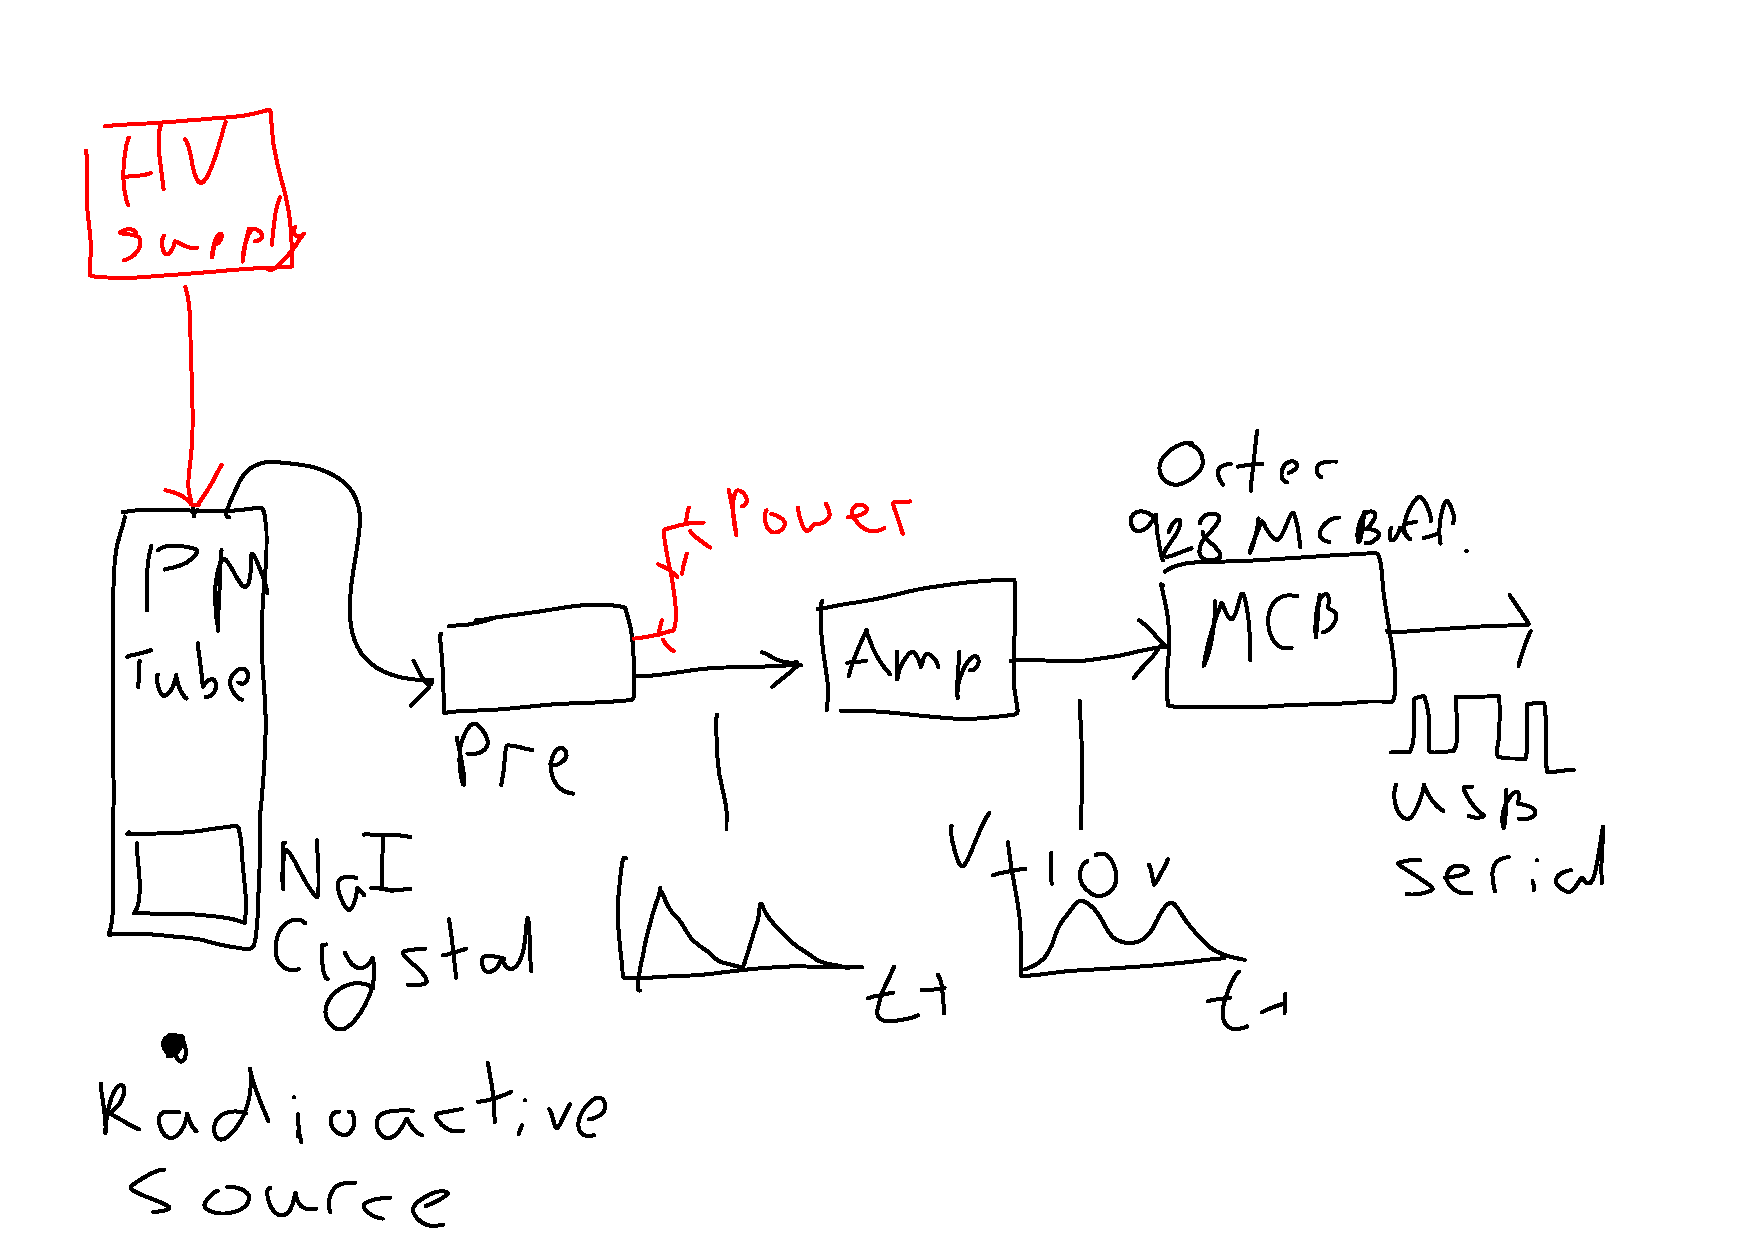
\includegraphics[width=0.6\textwidth]{figures/experiment-setup.pdf}
    \caption{Configuration of hardware for experiment. Raw signals originate at the Photo Multiplier Tube (PM Tube in figure), which is triggered by the radioactive source, which was placed approximately 3 cm in front of the PM Tube. These signals are fed into the Pre-Amplifier, (Pre Amp in figure), before passing into the amplifier. The signal has peaks at approximately 10 Volts after exiting the amplifier, where it is then fed into the Multi-Channel Buffer. Data from the Multi-Channel Buffer is analyzed on a computer via Spectrum32 software.}
    \label{fig:hardware-config}
\end{figure}

\section{Spectrum Analysis of $^{137}\mathrm{Cs}$, $^{22}\mathbf{Na}$, and $^{60}\mathrm{Co}$}

\textbf{Data saved at: }

\section{Spectrum and Half-life Measurement of Unknown Sample}

\textbf{Data saved at: }

\appendix
\section{NIM Setup}
\end{document}